\documentclass[a4paper]{article}
\usepackage{hyperref}
\usepackage{amsmath, amsthm, amssymb}
\usepackage[round]{natbib}
\usepackage{fullpage}
% The line below tells R to use knitr on this.
%\VignetteEngine{knitr::knitr}

\title{Fast Bayesian TDP Mixture Model Package}
\author{Xiaoyu Lu}

\usepackage{Sweave}
\begin{document}
\Sconcordance{concordance:vignettes.tex:vignettes.Rnw:%
1 11 1 1 0 17 1 1 2 1 0 2 1 1 2 1 0 3 1 1 4 6 0 1 2 1 1 1 2 1 0 4 1 4 0 %
1 2 2 1 1 14 1 2 3 1 1 2 1 0 1 7 6 0 1 4 6 0 1 2 1 3 5 0 1 2 2 1 4 0 1 %
3 4 1}

\maketitle
\begin{abstract}
This is a fast R Bayesian TDP mixture model package. The posterior distributions are obtained through Gibbs sampling, and the speed up is achieved through calling from C code and parallelization using OpenMP. The package can be found on https://github.com/xiaoyulu2014/Mixpack.
\end{abstract}
\section{Introduction}
In this project, we implement a Bayesian mixture model in R, with part of the codes in C for faster computation. It applies to multivariate data with any dimension. The speed can be slow in R if the data is large, therefore we coded the most expensive part of the R code in C to speed up. 


\section{Bayesian TDP mixture model}
The \emph{Truncated Dirichlet Process (TDP)} mixture model places a Normal-Inverse Wishart priors for normal component parameters, $i.e. (\mu_j, \Sigma_j) \sim  N(\mu_j|m,\gamma\Sigma_j)IW(\Sigma_j|\nu+2,\nu\Phi)$ independently over $j=1:k$, where $k$ is the number of components. The term TDP comes from the implicit priors over mixture probabilities arising from the underlying DP model, $i.e. \pi_1 = v_1, \pi_j = v_j\prod_{r=1}^{j-1}(1-v_j)$ for $j=2:k-1$ and $\pi_k = 1 - \sum_{j=1}^{k-1}\pi_j$, where $v_j \sim Be(1,\alpha)$ for $j=1:k-1$. For simplicity, we do not learn the hyperparameters $\{\alpha,m,\gamma,\nu,\Phi\}$. \\

We implemented a block MCMC algorithm successively resamples values of the parameters $\Theta = \{\mu_{1:k},\Sigma_{1:k},\pi_{1:k}\}$. The evaluation of the conditional configuration probabilities $\pi_j(x_i) = Pr(z_i=j|x_i,\Theta) \propto \pi_jN(x_i|\mu_j,\Sigma_j)$ is very expensive, therefore we have coded it in C to call from R. For faster computation, we also used OpenMP for multi thread computation.


\section{Toy Example}
We applied the model to the data simulated from the following code:
\begin{Schunk}
\begin{Sinput}
> library(mvtnorm)
> library(MCMCpack)
> mu = list()
> #cluster means
> mu[[1]] = c(5,1,2);mu[[2]]=c(-5,-1,-2);mu[[3]] = c(0,2,0)
> n = 1000    #number of data points
> pi = c(0.6,0.3,0.1)   #mixing proportions
> x = matrix(,n,3);index=c()    #generating data
> for (i in 1:n){
+   index[i] = sample(1:3,1,prob=pi)
+   x[i,] = mvrnorm(1,mu[[index[i]]],diag(3))  #identity covariance matrices
+ }
\end{Sinput}
\end{Schunk}

With 200 sampling steps and 150 burn-in period, the classification of these data points projected onto the first 2-d dimension can be found in the following plot:
\begin{Schunk}
\begin{Sinput}
> K=5   #initializing the number of clusters
> require(GPUmix)
> res = MCMC(x,K,200,150)
> plot(x,col=index)
> points(x,col=res$z)
\end{Sinput}
\end{Schunk}
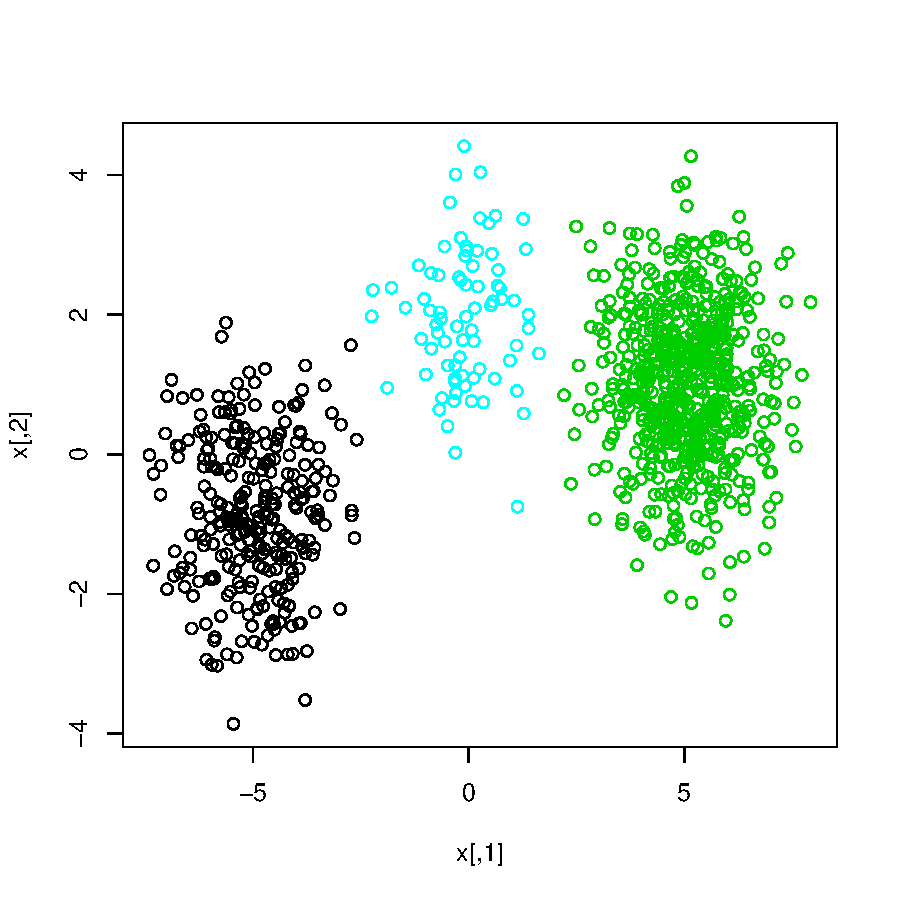
\includegraphics{vignettes-chunk3}

Different color corresponds to different clusters, the model has found the correct number of clusters and has classcified all data points correctly. The histogram of components of x and 1000 data generated from the learned parameters can be found below:\\

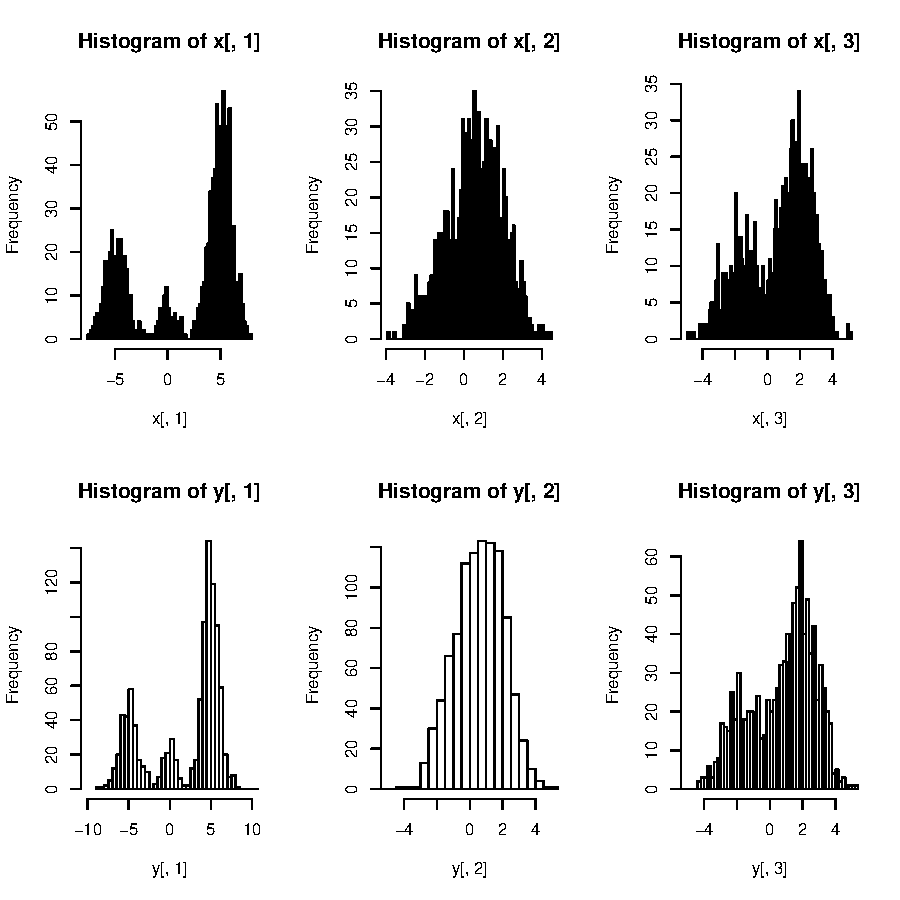
\includegraphics{vignettes-chunk4}

\section{Calling from C and OpenMP}
The accuracy of the model is good, and now we wish to reduce the computational time by replacing the code below:

\begin{Schunk}
\begin{Sinput}
> out = c()
> pdf_func = function(x,pi,mu,Sigma) {
+   for (j in 1:K){
+     out[j] = pi[j] * dmvnorm(x,mu[[j]],Sigma[[j]])       
+   }
+   out = out/sum(out)   
+   return(out)
+ }
> for (i in 1:nr) {       
+   pdf = pdf_func(x[i,],pi,mu,Sigma)
+   z[i] = which.max(pdf)
+   }
\end{Sinput}
\end{Schunk}
with
\begin{Schunk}
\begin{Sinput}
> z = .C("mixpdf", as.integer(nr),as.integer(K), as.integer(nl), as.double(pi), as.double(t(x))
+  ,as.double(unlist(mu)), as.double(unlist(Sigma)), result = as.double(rep(0,nr)))$result + 1
\end{Sinput}
\end{Schunk}

This has improved the running time dramatically with the toy dataset in Section 3. To further improve it, we used OpenMP:
\begin{Schunk}
\begin{Sinput}
> #pragma omp parallel for 
\end{Sinput}
\end{Schunk}

The timing of the C code can be founs in timer.c. However, using OpenMP in this case does not give an improvement, this is likely due to the communication cost between the threads.


\end{document}
